\section{Durchführung}
\label{sec:Durchführung}

\subsection{Aufbau}
Für den Versuch wird eine Neutronenquelle aus einem Gemisch aus $^6Be$ und $^{226}Ra$ verwendet. Die Neutronen werden in der Apperatur abgebremst,
sodass ihre Geschwindigkeit gleich der mittleren kinetischen Energie der sie umgebenen Moleküle bei Raumtemperatur ist.
Die verlangsamten, thermischen Neutronen werden dann auf einen Verstärker gerichtet, welcher einen konstanten Bruchteil der Zerfälle misst.
Über zwei Zähler, welche in einem konstanten Zeitintervall abwechselnd messen, können dann die Anzahl der Zerfälle abgelesen werden.
Der tatsächliche Versuchsaufbau ist in Abbildung \ref{fig:tatVersuch} gezeigt.

\begin{figure}
    \centering
    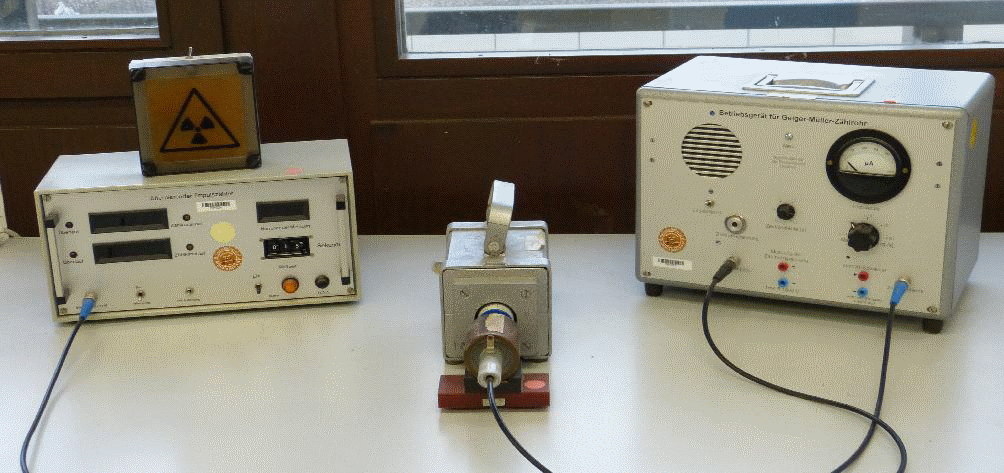
\includegraphics[width=.9\textwidth]{plots/tatVersuch.png}
    \caption{Tatsächlicher Versuchsaufbau.\cite{Versuchsanleitung}}
    \label{fig:tatVersuch}
\end{figure}

Die Probe inklusive der Neutronenquelle sind in einem Bleischirm gehüllt, um ausgehende Strahlung und den Nulleffekt, welcher durch Höhenstrahlung und natürlicher Radioaktivität verursacht wird,
zu minimieren.
Der Versuch ist vollständig aufgebaut, wenn die einzelnen Elemente wie in Abbildung \ref{fig:tatVersuch} aufgestellt und verkabelt sind.
Abbildung \ref{fig:schVersuch} zeigt den schematischen Aufbau der Apperaturen.

\begin{figure}
    \centering
    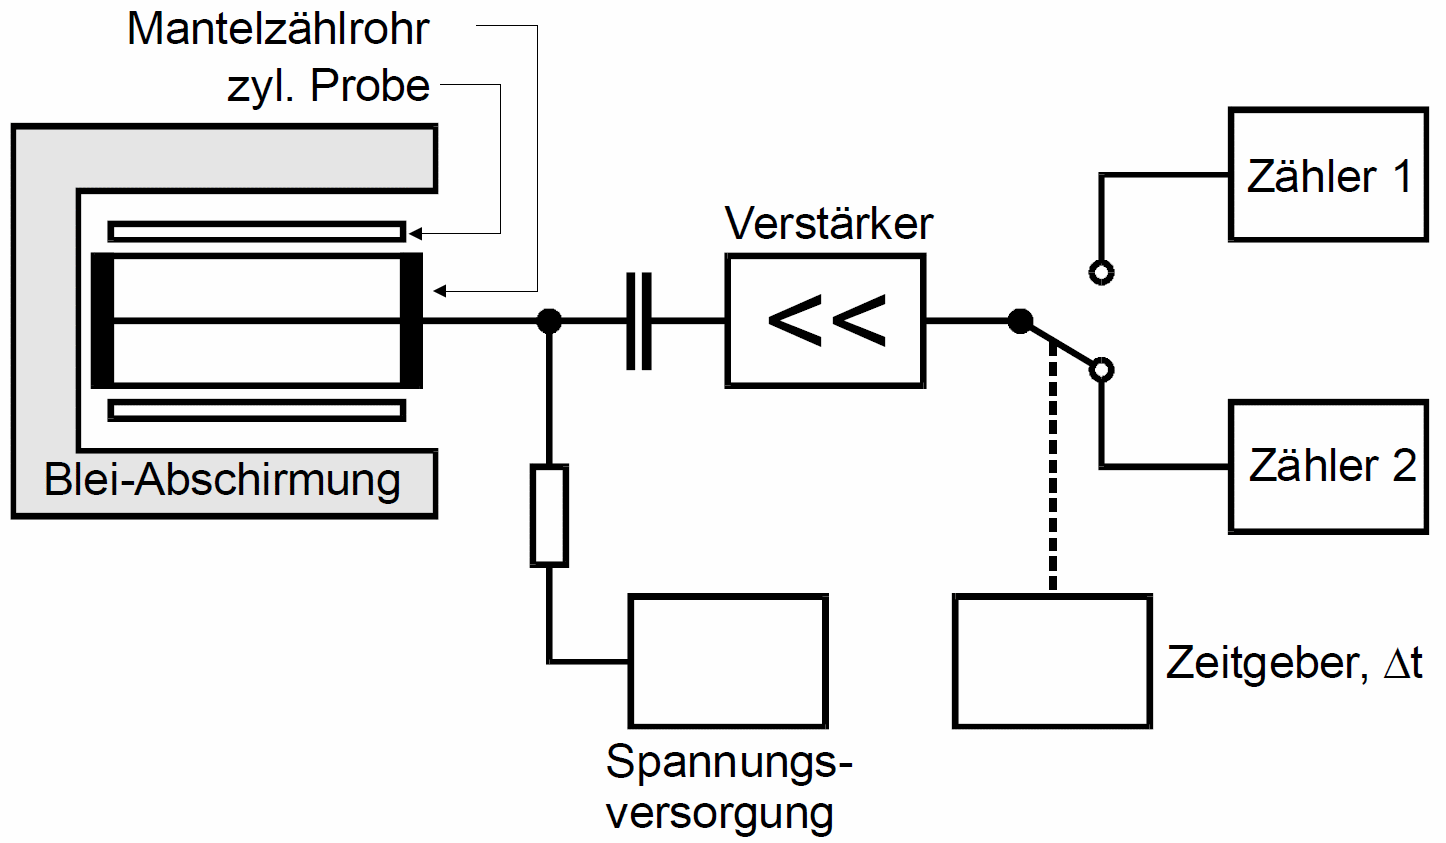
\includegraphics[width=.9\textwidth]{plots/Versuch.png}
    \caption{Schematischer Versuchsaufbau.\cite{Versuchsanleitung}}
    \label{fig:schVersuch}
\end{figure}

\subsection{Messung des Nulleffekts}
Um den Nullefekt zu messen, wird die aktivierte Neutronenquelle auf den Verstärker gerichtet und die Anzahl der Zerfälle abgelesen.
Der relative Fehler wird minimiert, indem die Messung bei einem Zeitintervall von $\SI{300}{\second}$ sieben mal wiederholt wird.

\subsection{Messreihen für Vanadium und Rhodium}
Entscheidend ist die Wahl des Zeitintervalls für die einzelnen Zerfallsmessungen. Durch Ausprobieren ergeben sich optimale Zeitintervalle, welche für $^{52}V$ bei $\Delta t = \SI{30}{\second}$
und für $^{104}Rh$ bei $\Delta t = \SI{15}{\second}$ liegen.

Die zylindrischen Proben werden in die Neutronenquelle eingeführt und die Apperatur auf den Verstärker ausgerichtet. An dem Zähler wird das entsprechende Zeitintervall eingestellt
und direkt nach Einführen der Probe abgelesen.
Für jedes Element werden 42 Zeitintervalle gemessen.